%%%%%%%%%%%%%%%%%%%%%%%%%%%%%%%%%%%%%%%%%
% Thin Sectioned Essay
% LaTeX Template
% Version 1.0 (3/8/13)
%
% This template has been downloaded from:
% http://www.LaTeXTemplates.com
%
% Original Author:
% Nicolas Diaz (nsdiaz@uc.cl) with extensive modifications by:
% Vel (vel@latextemplates.com)
%
% License:
% CC BY-NC-SA 3.0 (http://creativecommons.org/licenses/by-nc-sa/3.0/)
%
%%%%%%%%%%%%%%%%%%%%%%%%%%%%%%%%%%%%%%%%%

%----------------------------------------------------------------------------------------
%	PACKAGES AND OTHER DOCUMENT CONFIGURATIONS
%----------------------------------------------------------------------------------------

\documentclass[a4paper, 11pt]{article} % Font size (can be 10pt, 11pt or 12pt) and paper size (remove a4paper for US letter paper)

\usepackage[protrusion=true,expansion=true]{microtype} % Better typography
\usepackage{graphicx} % Required for including pictures
\usepackage{wrapfig} % Allows in-line images
\usepackage{amsmath}
\usepackage{amsfonts}
\usepackage{amssymb}
\usepackage{algpseudocode}
\usepackage{listings}
\usepackage{color}
\usepackage{caption}
\usepackage{subcaption}
\usepackage{float}
\usepackage{mathpazo} % Use the Palatino font
\usepackage[T1]{fontenc} % Required for accented characters
\linespread{1.05} % Change line spacing here, Palatino benefits from a slight increase by default
\usepackage{url}
\makeatletter
\renewcommand\@biblabel[1]{\textbf{#1.}} % Change the square brackets for each bibliography item from '[1]' to '1.'
\renewcommand{\@listI}{\itemsep=0pt} % Reduce the space between items in the itemize and enumerate environments and the bibliography

\renewcommand{\maketitle}{ % Customize the title - do not edit title and author name here, see the TITLE block below
\begin{flushright} % Right align
{\LARGE\@title} % Increase the font size of the title

\vspace{50pt} % Some vertical space between the title and author name

{\large\@author} % Author name
\\\@date % Date

\vspace{40pt} % Some vertical space between the author block and abstract
\end{flushright}
}

%----------------------------------------------------------------------------------------
%	TITLE
%----------------------------------------------------------------------------------------

\title{\textbf{Advances in Data Mining}\\ % Title
Assignment 1: Locality Sensitive Hashing} % Subtitle

\author{\textsc{Giulio Lovisotto - s1595687 \\ Daniele Lain - s1602403} % Author
\\{\textit{Institute of Advanced Computer Science, Leiden}}} % Institution

\date{October 20, 2014} % Date

%----------------------------------------------------------------------------------------

\begin{document}

\maketitle % Print the title section

%----------------------------------------------------------------------------------------
%	ABSTRACT AND KEYWORDS
%----------------------------------------------------------------------------------------

%\renewcommand{\abstractname}{Summary} % Uncomment to change the name of the abstract to something else

\begin{abstract}
In this report we summarize our results for the main task of the  Assignment 1 of the course of Advances in Data Mining.
We applied text mining techniques to a dataset formed by the lyrics from the songs of the \textit{Million Song Dataset}, namely \textit{musiXmatch}, to find similarities and to check whether there are correlations among the lyrics of songs of the same genre. We found that lyrics alone are not a sufficient parameter to discriminate between genres, but could still prove to be useful in broader music analysis.
\end{abstract}

\vspace{20pt} % Some vertical space between the abstract and first section

%----------------------------------------------------------------------------------------
%	ESSAY BODY
%----------------------------------------------------------------------------------------

\section{Introduction}

%------------------------------------------------

the \textit{Million Song Dataset} \cite{MSDS} is a collection of audio features and metadata for a million contemporary popular music tracks. The \textit{musiXmatch} \cite{MXM} dataset is an accompanying lyrics database, providing bag-of-words lyrics to over 260.000 songs of the original dataset.
We check whether these lyrics could be an useful parameter to classify songs into different genres.

 This approach was suggested by Logan, Beth and Kositsky, who found lyrics analysis itself to be less accurate that acoustic analysis, but showed how clustering could be helped by this feature \cite{logan2004semantic}. Liang, Gu et al. used lyrics and acoustic features using the Million Song Dataset itself \cite{liang2011music}, and their work was extended by Bou-Rabee who used it to train several learners which obtained a fairly high accuracy, between 50\% and 65\% \cite{bourabee}.

We compute various similarity measures between the bag-of-words lyrics of the dataset and then check our findings against a ground truth we obtained for a subset of the data.\\

The rest of the report is organized as follows: in section 2 we report the structure of the dataset and the preprocessing of the data we do to obtain the final test suite, in section 3 we describe the algorithms and the methodology used to compute the metrics and to obtain the results, in section 4 we show and analyze the results and in section 5 we draw conclusions on the work.


%------------------------------------------------

\section{Dataset}

For our work we had to combine the information contained in two different datasets, because we needed to obtain both the lyrics of a song and its genre. The datasets we used are the \textit{musiXmatch} \footnote{musiXmatch dataset, the official lyrics collection for the Million Song Dataset, available at: http://labrosa.ee.columbia.edu/millionsong/musixmatch} dataset and the \textit{MSD genre} \footnote{MSD genre dataset, available at: http://labrosa.ee.columbia.edu/millionsong/blog/11-2-28-deriving-genre-dataset} dataset which are briefly described.
\subsection*{musiXmatch}
This dataset contains the official collection of lyrics for the songs in the \textit{Million Song Dataset}. The dataset is composed of the lyrics for only 237,662 tracks, since some were not released for various reasons. The lyrics come in bag-of-words format: each track is described as the word-counts for a dictionary of the top 5,000 words across the whole set. The dataset is distributed as a .txt file where every line is formatted as follows: 
\begin{center}<\textit{track\_id, MXMID, idx:cnt, idx:cnt,}...> \end{center}
where \textit{track\_id} is the track id in the \textit{MSD}, \textit{MXMID} is the id in the \textit{musiXmatch} dataset, and the pairs \textit{idx:cnt} are the occurrences of word of index \textit{idx} in this track. \\
Along with the dataset comes the full list of stemmed words and the total word counts There are 498,134 unique words, for a total of 55,163,335 occurrences. The 5,000 words in the dataset account for 50,607,582 occurrences, so roughly 92\%. In order to choose the first 5,000 words, the word counts was normalized by the number of word occurrences in each song. The list of words is distributed as a .txt file where every line is formatted as follows:
\begin{center}<\textit{word, occurrences}> \end{center}
the file is already sorted, the most frequent words are at the top of it.
There is a non-stemmed version available on the website, but since the stemming procedure does not significantly change the overall result we just tested our results on the stemmed version.
\subsection*{MSD genre}
This dataset contains a classification of the songs from the \textit{MSD} by genre. The dataset contains the genre for 59,600 tracks. The dataset was built using the \textit{musicbrainz} tags that describe typical genres. Since they were applied by humans, they are consistent and descriptive.\\
The dataset contains the following ten genres: classic pop and rock, folk, dance and electronica, jazz and blues, soul and reggae, punk, metal, classical, pop, hip-hop. \\
The dataset also contains a set of features obtained from The Echo Nest, which are: loudness, tempo, time\_signature, key, mode, duration, average and variance of timbre vectors, but in our work we'll ignore them since they are not in the scope of our problem. \\
The dataset is distributed as a .txt file where every line is formatted as follows:
\begin{center}<\textit{genre, track\_id, artist\_name, title, loudness, tempo, time\_signature,}...> \end{center}
where \textit{genre} is a string containing one of the 10 genres listed above, and \textit{track\_id} is the id of the track in the \textit{MSD}. \\
The authors point out that the dataset is simplified, and the main problem is the unbalancedness of the data (the tracks are not distributed uniformly among the genres), but in our opinion this is suitable for our implementation to yield a meaningful result.
\subsection*{Categorizing Documents}
To correctly apply our methods we needed to purify our dataset from the words that were not meaningful in the document, and moreover we also needed to rank the words based on their importance, since a bag composed of 5,000 words might be too large and then non significant in our analysis. For this purpose we did the following:
\begin{itemize}
\item Remove \textbf{stop words: } words that are very common in English so it's a good practice to remove them before processing documents;
\item Calculate \textbf{TFIDF:} for every word we calculated its importance using the TFIDF value
\end{itemize}
\subsection*{Joining the datasets}
For our purpose we combined the information contained in the two datasets to build a single database, using the python scripts provided by the authors of the datasets on the website. A slightly customized version of the provided script \textit{mxm\_dataset\_to\_db.py} is used to build a SQLite database for convenience of use, another script \textit{fill\_genres.py} is used to look up for the genres on the \textit{MSD genre} dataset and add them to our database, then \textit{cleanup.py} removes all non-classified tracks (tracks that have no genres in the other dataset), removes all the stop-words, and removes the table \textbf{words} that we don't need, and in the end \textit{tfidf.py} loops on the records and calculates the TFIDF for every word. \\
The result of the import process is a SQLite database which contains a single table \textbf{lyrics} which has 933,569 rows (one per word per song) for 17,594 tracks divided into 10 genres, and contains the following fields:
\begin{enumerate}
\item \textbf{track\_id:} string, contains the id of the track in the \textit{MSD} 
\item \textbf{mxm\_tid:} string, contains the id of the track in the \textit{musiXmatch} database
\item \textbf{word:} string, the word considered by this record
\item \textbf{count:} int, the number of occurrences of word in this song
\item \textbf{is\_test:} int, indicates whether this track is part of the train dataset or of the test dataset (we ignore this field)
\item \textbf{genre:} string, the genre for this song
\item \textbf{tfidf:} float, the TFIDF for this word
\end{enumerate}
This is not the cleanest model for the data structure, because of the great redundancy, but since we don't need to operate on the data but just to read them we sticked with the structure the mantainers of the dataset decided.
Because of timing constraints and convenience we picked (for most of the computations) 2,144 of the 17,594 tracks. Since the selection was uniformly distributed among genres, we believe that this does not bias the dataset and that the results are still informative.

%----------------------------------------------------------------------------------------
%	BIBLIOGRAPHY
%----------------------------------------------------------------------------------------
\section{Metodology}
\subsection*{Computations} Our primary goal was to understand if the lyrics of a song are a good criterion to discriminate among genres. We then computed the following measures:
\begin{enumerate}
	\item \textbf{Jaccard similarities: } since the dataset size was manageable, we computed the Jaccard similarity on the bag-of-words over all the pairs of songs in our dataset. Moreover, we computed the Jaccard similarity between bag-of-words of fixed length, picking the $m$ most significant words for every track (using the \textit{tfidf} measure), to check whether using a fixed size set (discarding words of minor importance for every given song) altered the results and how.
	\item \textbf{Minhash: } we computed the minhash signatures for all the songs. We used $k = 720$ hash functions both because it allowed us to study different configurations for $b$ and $r$ when appying the banding technique, and because we believe it's a good value for our dataset, since the average different word count for every song is about $50$ (with slight differences among distinct genres).
	\item \textbf{Signatures similarities: } using the minhash signatures we computed the signature similarities $\left(\frac{\text{\# identical elements}}{\text{signature length}}\right)$ between them.
\end{enumerate}
\subsection*{Modus Operandi}
We used the computed results as follows:
\begin{enumerate}
	\item \textbf{General Pattern: }Since we had the ground truth for the classification (given in our genre dataset), we could compare it to the output of a similarity measure. We used this algorithm:
	
	\hrulefill
	\begin{algorithmic}
		\For {$(S_i, S_j)$ in $songs$}
			\State $\text{js = } similarity_{i,j}$
			\If {$js \geq threshold$}
				\State $\text{check if songs are in the same genre}$
			\Else
				\State $\text{check if songs are not in the same genre}$
			\EndIf
		\EndFor
	\end{algorithmic}
	\hrulefill
	
	to compute the result of the classification of the tracks given a similarity measure between them.\\
	
	The algorithm allowed us to find the number of true positives, true negatives, false positives, false negatives. We were interested in studying the values for the following measures:
	\begin{itemize}
		
		 \item \textbf{Precision}: true positives divided by true and false positives;
		 \item \textbf{Recall}: true positives divided by true positives and false negatives;
		 \item \textbf{Accuracy}: true positives and negatives divided by the total cardinality;
		 \item \textbf{Specificity}: true negatives divided by false positives and true negatives.
	\end{itemize}	
		 
	We computed the values for the above mentioned measures for 
	\begin{itemize}
	 	\item varying threshold $s$ for Jaccard similarity;
	 	\item varying bag of words sizes, picking the $n$ highest tfidf words for every track
	 	\item varying configuration of $b, r$ for the banding technique applied to the minhash signatures;
	 	\item the signature similarity.
	\end{itemize}
	\item \textbf{Histogram of similarities: }We computed the histogram of similarities containing the number of same-genre songs that were similar for varying values of the similarity. This allowed us to see whether the lyrics are a good feature for discriminating between genres. We studied this both for Jaccard similarity and for signature similarity.
\end{enumerate}

\subsection*{Technologies}
The work was developed in python version 2.7.3. We used the python module sqlite3 to interact with the SQLite database where we stored the results of long computation processes. We used the matplotlib.pyplot module to plot our results.

\newpage
\section{Results}

\begin{figure}[h]
\centering
\noindent\makebox[\textwidth]{%
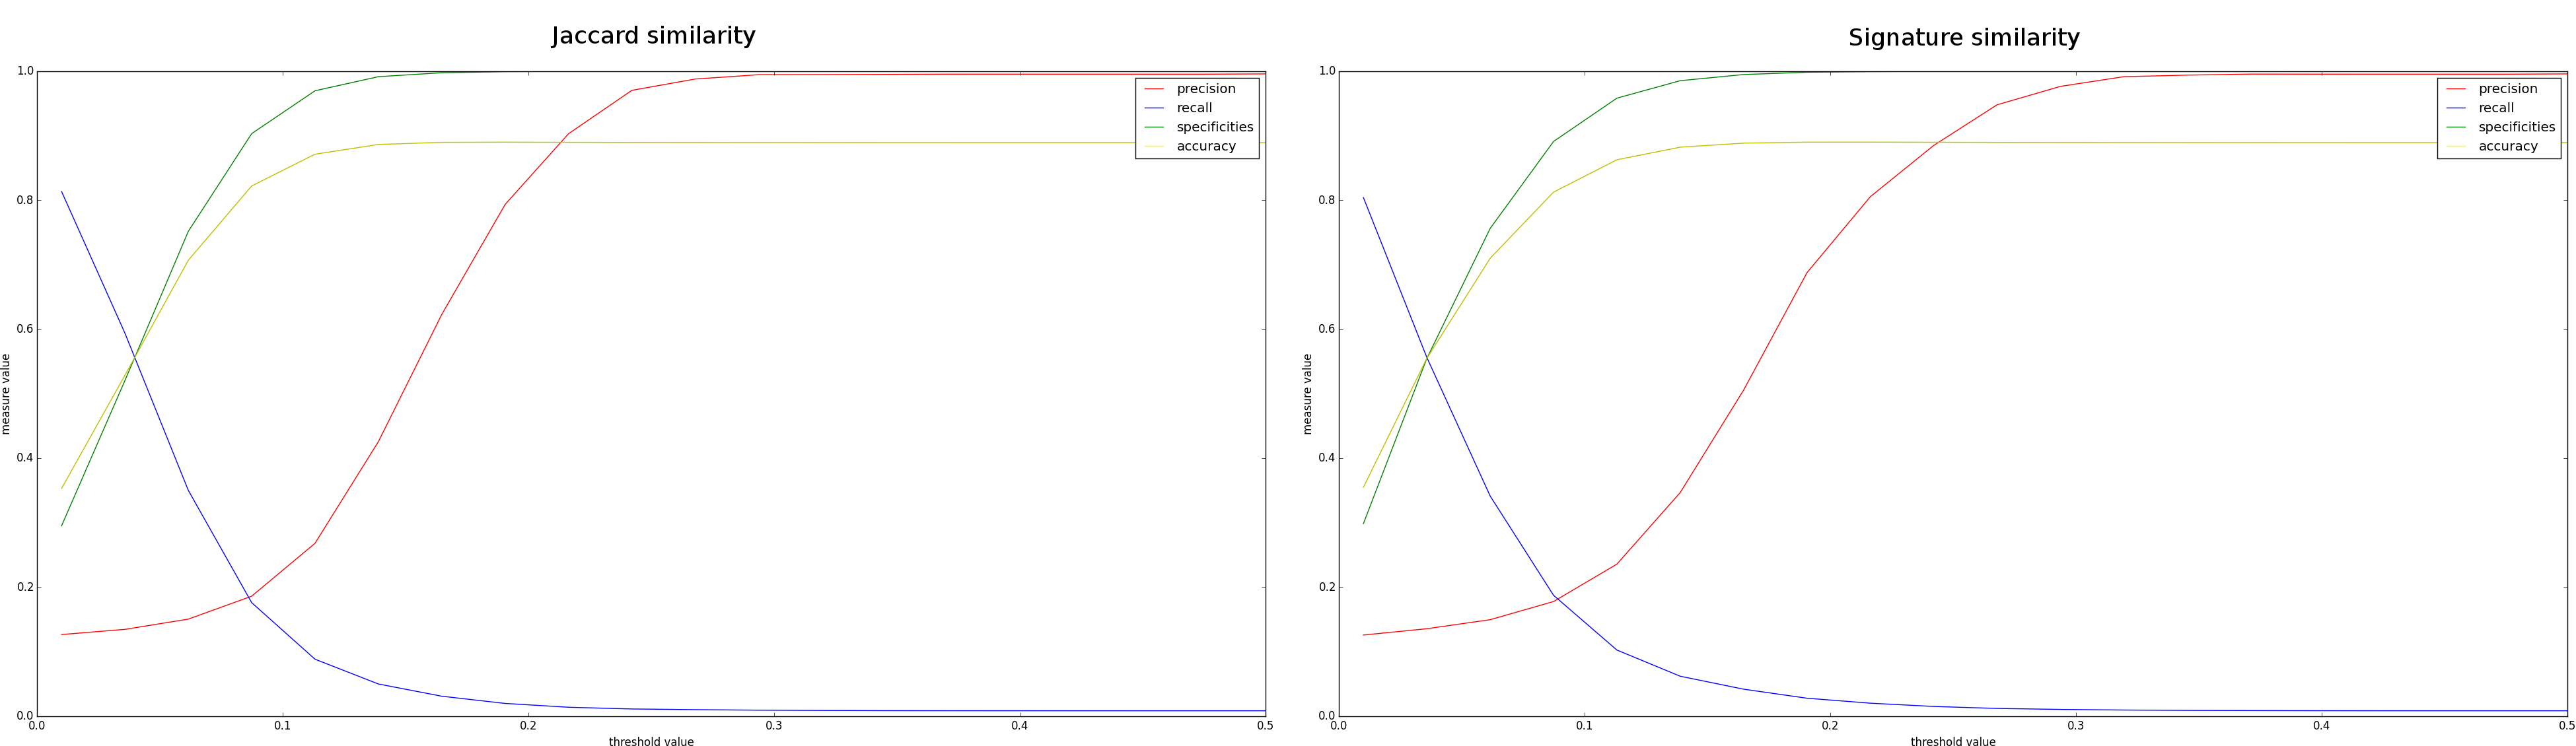
\includegraphics[width=1.5\textwidth]{images/ad}
}
\caption{Measures on different treshold values. The left plot uses the Jaccard similarity, the right plot uses similarity between signatures}
\label{fig:ad}
\end{figure}

We can see how the exact and approximate method led to almost identical results, showing that the signature technique is a good approximation of the Jaccard similarity. The results show that the best compromise of precision and recall is when the threshold is at around 0.1, and even then our system gets an approximate 20\% of correct answers.
This is better than a random selection, but it is not too high and already shows that lyrics can be a complementary parameter on which we cannot rely alone. 

From these results we expect then the banding technique we perform to get the best results when the theoretical threshold is around 0.1. This can be obtained with 360 bands of 2 elements (expected $s=0.052$) and 240 bands of 3 elements (expected $s=0.16$).\\ 
\begin{figure}[H]
\centering
\noindent\makebox[\textwidth]{%
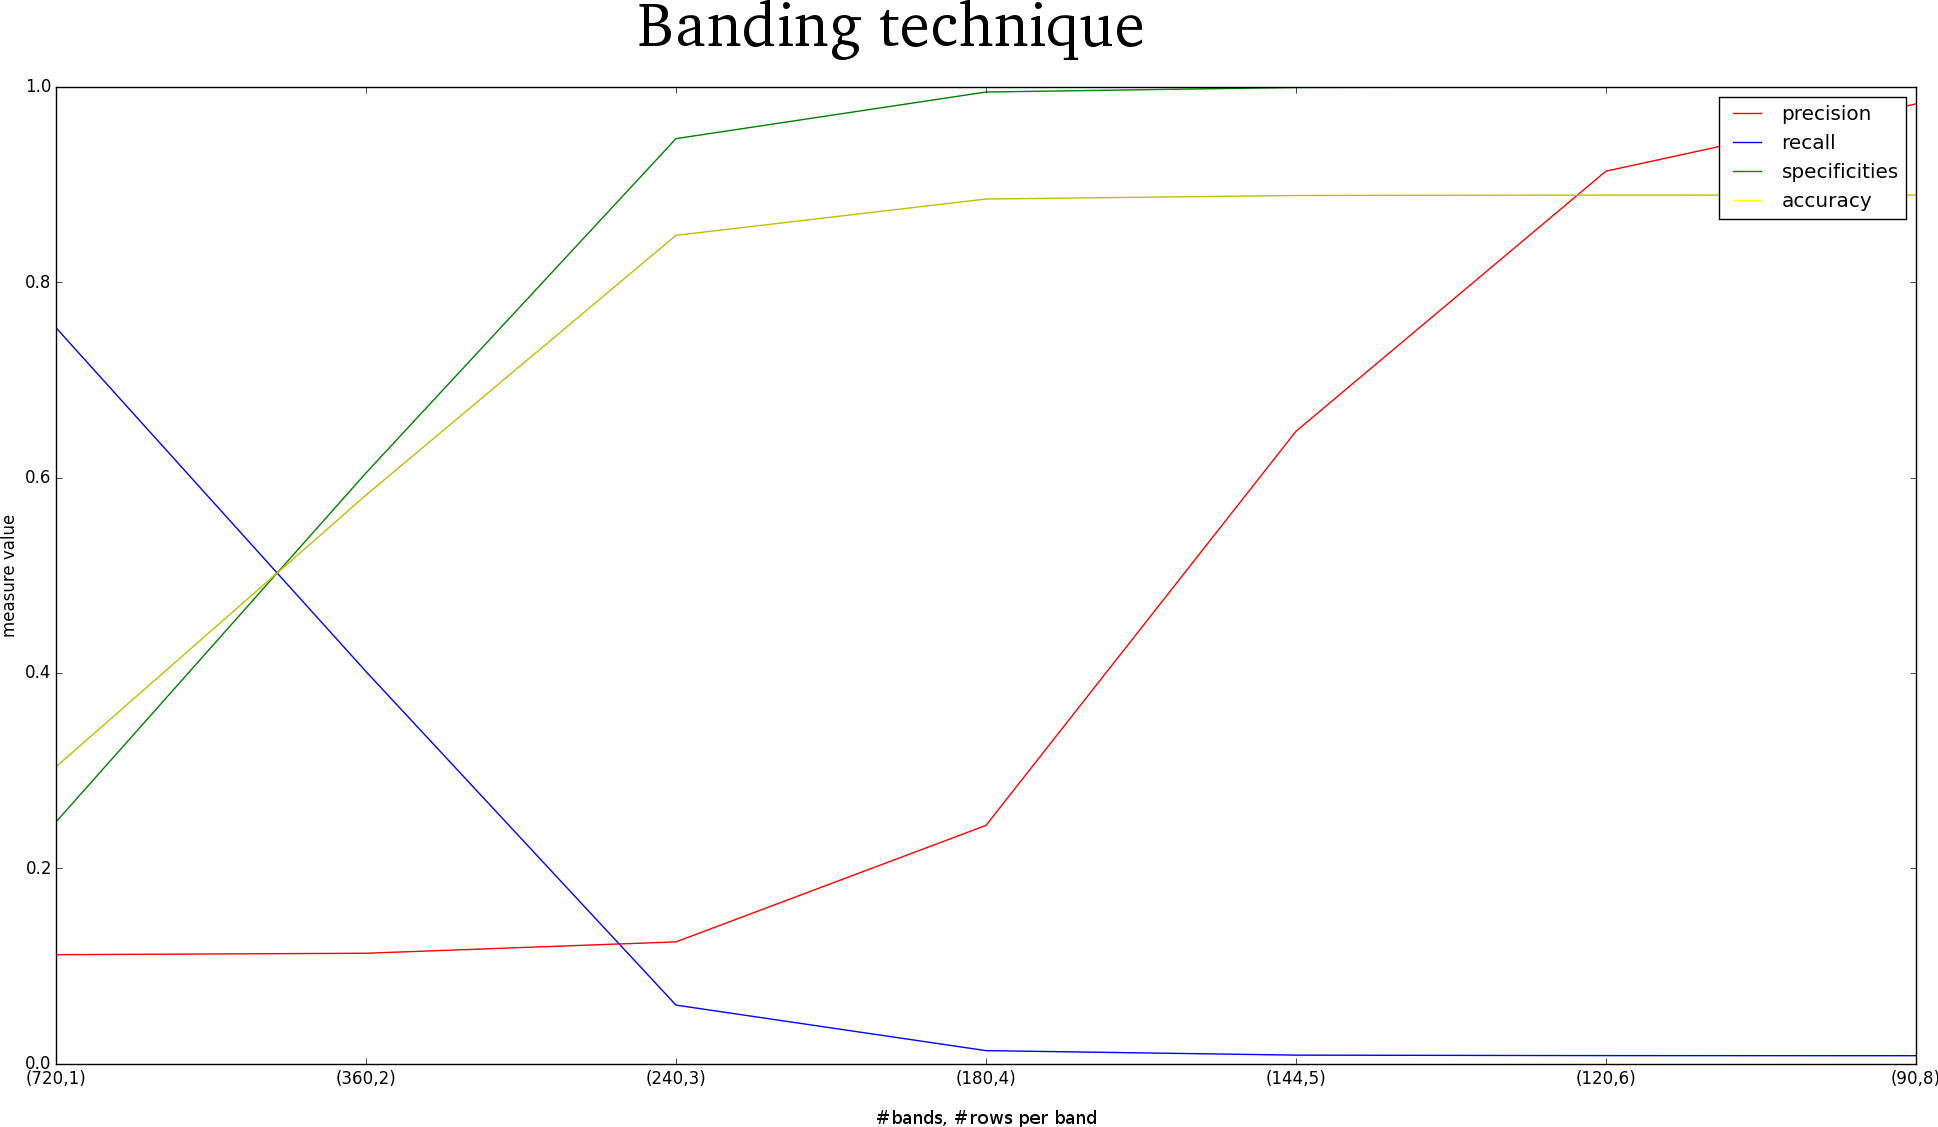
\includegraphics[width=\textwidth]{images/c_edited}
}
\caption{Measures on different parameters (b, r) for the banding technique.}
\label{fig:c}
\end{figure}
In this chart we see that the curves, even though they are more discrete, resemble the ones found in figure \ref{fig:ad}, which means that the minhash and banding techniques are working correctly. We can see that the curves follow the same pattern, in particular the value for the precision starts to rise and the recall goes low for $b=240, r=3$ which means with a theoretical threshold of $s=\frac{1}{b}^{\frac{1}{r}} \sim 0.16$, which is consistent with our previous result.

\begin{figure}[H]
\centering
\noindent\makebox[\textwidth]{%
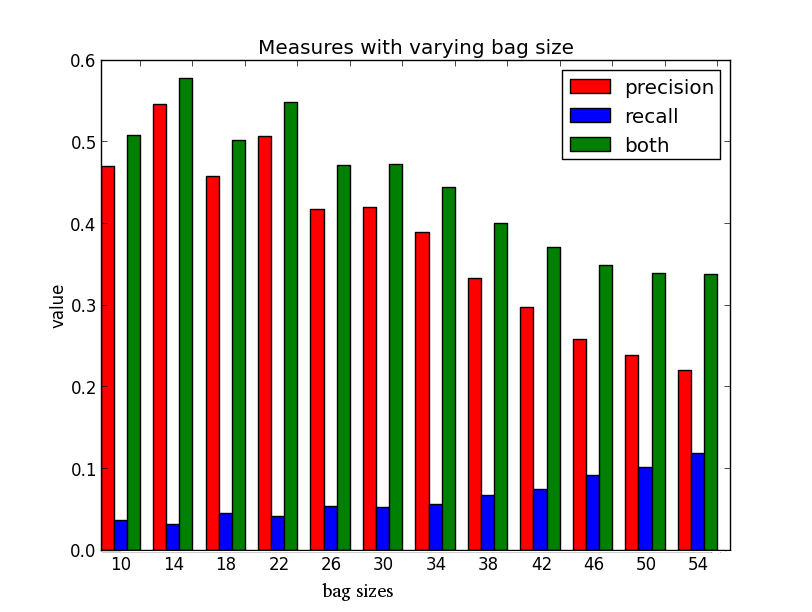
\includegraphics[width=\textwidth]{images/b_edited}
}
\caption{Precision and Recall for different bag of word sizes, using the first $n$ words with the highest TFIDF}
\label{fig:b}
\end{figure}
With this chart we wanted to check whether using a smaller set of most significant words for every track altered the classification result. Since the average number of words per song is about 50, we chose the sizes to be equally spaced integers between 10 and 54. The threshold $s$ for this chart is fixed at $0.08$, which is the best compromise between precision and recall we found experimentally.\\
We can see that using a smaller word set increases the precision but lowers the recall, and vice versa, which means that with small bag sizes we have a low number of false positives, but a high count of false negatives. This means that considering the whole set of words is a best approach to compute the similarities, since different tracks have only a few terms in common.


\begin{figure}[H]
\centering
\noindent\makebox[\textwidth]{%
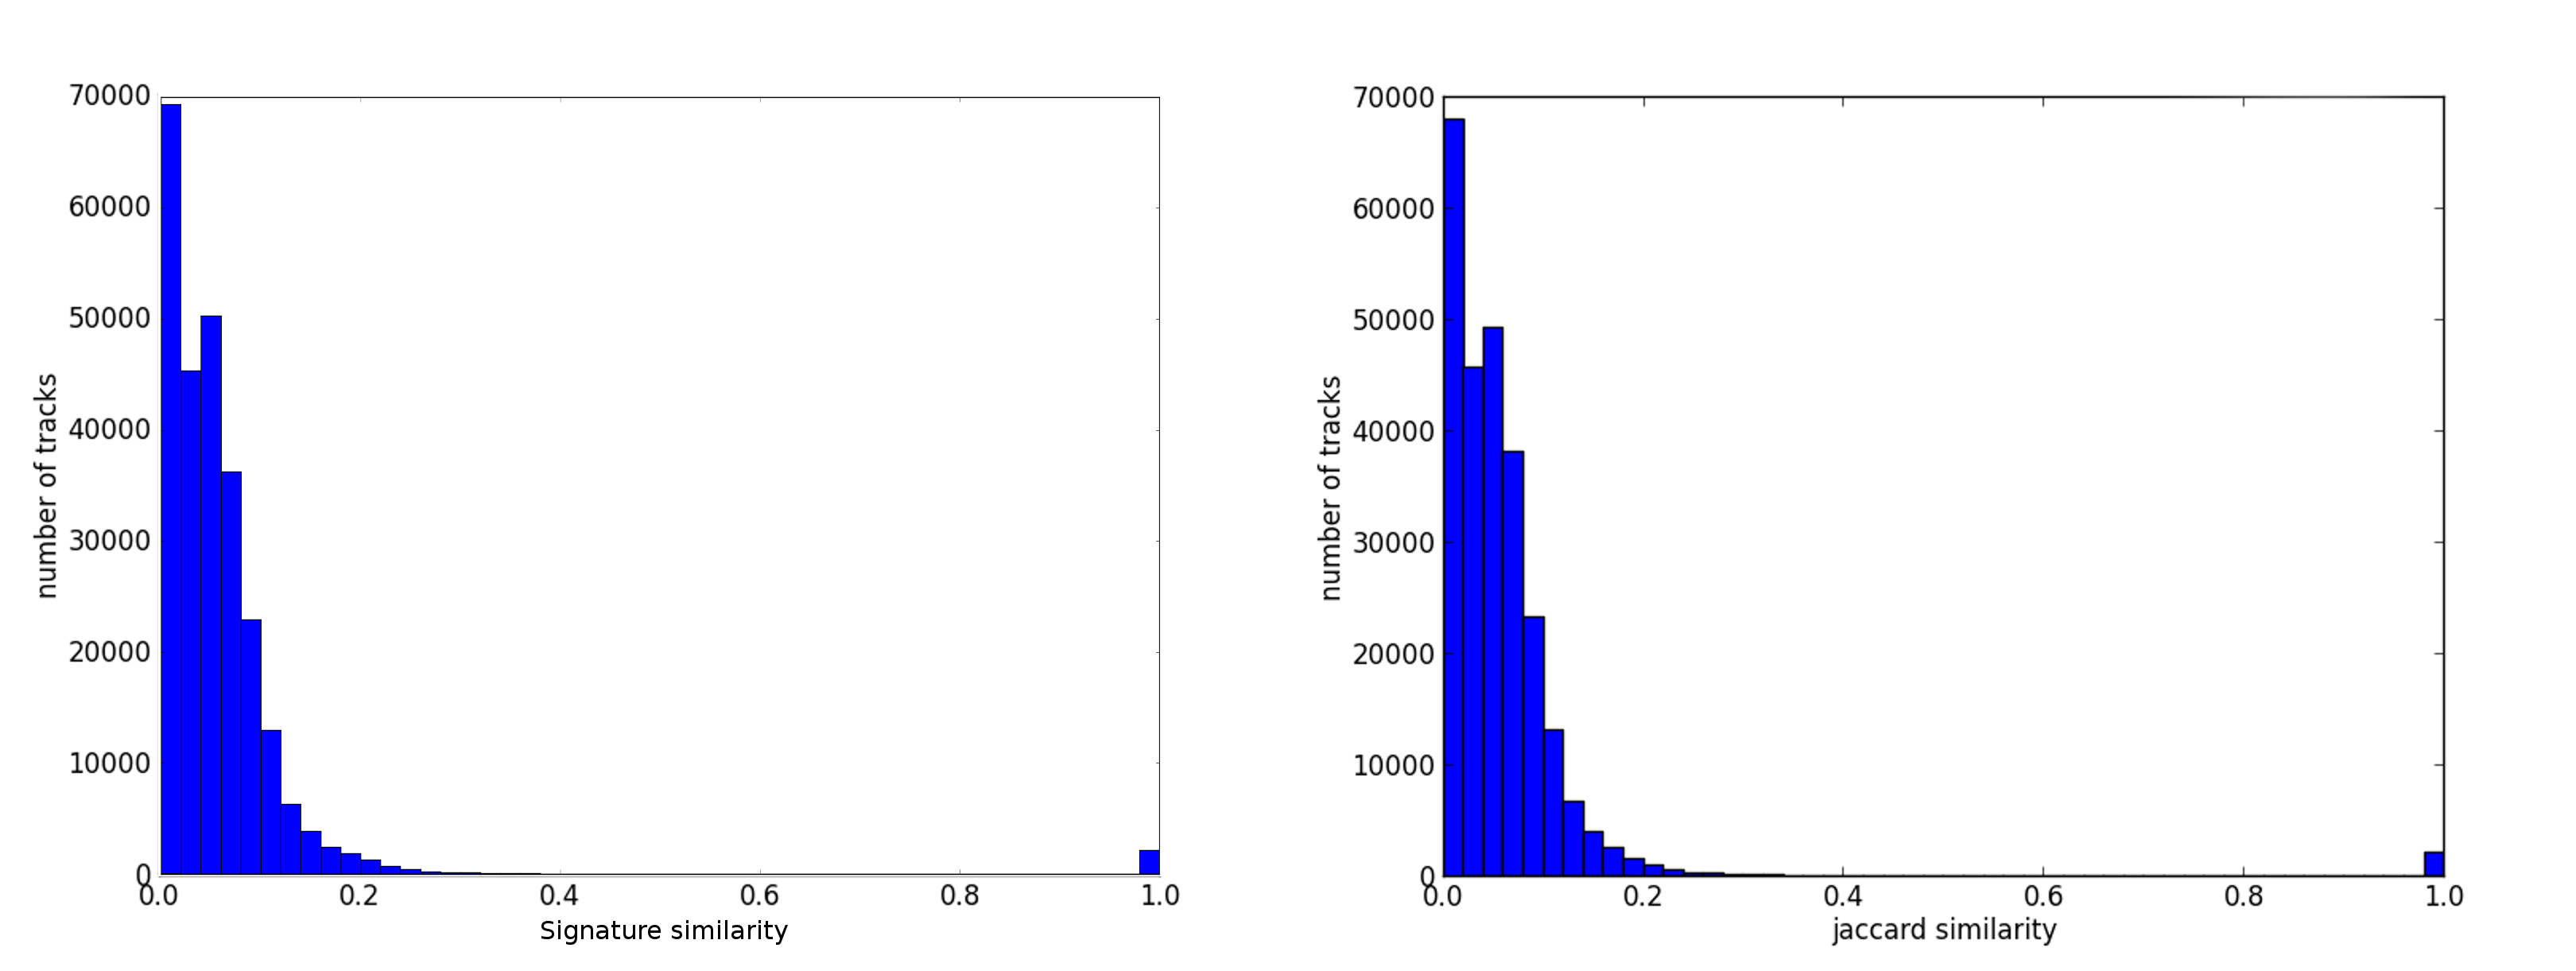
\includegraphics[width=1.5\textwidth]{images/ef}
}
\caption{Similarity distribution in the dataset. The left plot uses the signature similarity, the right one the Jaccard similarity}
\label{fig:ef}
\end{figure}
This plots shows how similar are songs belonging to a same genre. We computed the signature similarity and Jaccard similarity between all pairs of songs, and then we kept only the pairs where the song had the same genre. We then plotted the histogram of similarities, therefore we can see how many couples of same-genre tracks have a given similarity value.

We can see that more than 90\% of the similarities lies in range $(0, 0.2)$. This means that most of the songs have only a few words in common which makes the lyrics themselves not a very sound feature to use to discriminate between genres. This also gives good explanation of the precision and recall values we found, showing that they were somehow "expectable" - i.e. they are low because the similarity of the bag of words of songs of the same genre is usually very low.

\section{Conclusions}
We believe that the results we found show that song lyrics could be helpful as a feature to discriminate between song genres, but are not enough when used alone. The overall similarity is very low, this suggests that lower granularities in the similarity could be investigated. Moreover, an approach based on sentiment analysis of the bag-of-words, as suggested by Liang, Gu and O'Connor \cite{liang2011music}, creating sets of sentiments over which to perform the data mining, could be a more effective approach.



\bibliographystyle{unsrt}

\bibliography{sample}

%----------------------------------------------------------------------------------------

\end{document}